\documentclass[10pt,journal,compsoc]{IEEEtran}


\newtheorem{lemma}{Lemma}
\newtheorem{proposition}{Proposition}
\newtheorem{definition}{Definition}
\newtheorem{observation}{Observation}
\newtheorem{claim}{Claim}
\newtheorem{theorem}{Theorem}
\newcommand{\proof}[1]{{\em Proof}}

\newcommand{\Oh}[1]
  {\ensuremath{\mathcal{O}\!\left( {#1} \right)}}
\newcommand{\forward}
  {\ensuremath{\mathsf{forward}}}
\newcommand{\backward}
  {\ensuremath{\mathsf{backward}}}
\newcommand{\lastchar}
  {\ensuremath{\mathsf{lastchar}}}
\newcommand{\shorter}
  {\ensuremath{\mathsf{shorter}}}
\newcommand{\longer}
  {\ensuremath{\mathsf{longer}}}
\newcommand{\maxlen}
  {\ensuremath{\mathsf{maxlen}}}
\newcommand{\rank}
  {\ensuremath{\mathsf{rank}}}
\newcommand{\select}
  {\ensuremath{\mathsf{select}}}
\newcommand{\rsucc}
  {\ensuremath{\mathsf{succ}}}
\newcommand{\nodelabel}
  {\ensuremath{\mathsf{label}}}


\newcommand{\ignore}[1]{}

% *** CITATION PACKAGES ***
\ifCLASSOPTIONcompsoc
  % IEEE Computer Society needs nocompress option
  % requires cite.sty v4.0 or later (November 2003)
  \usepackage[nocompress]{cite}
\else
  % normal IEEE
  \usepackage{cite}
\fi

% *** GRAPHICS RELATED PACKAGES ***
\ifCLASSINFOpdf
  \usepackage[pdftex]{graphicx}
  % declare the path(s) where your graphic files are
  % \graphicspath{{../pdf/}{../jpeg/}}
  % and their extensions so you won't have to specify these with
  % every instance of \includegraphics
  \DeclareGraphicsExtensions{.pdf,.jpeg,.png}
\else
  % or other class option (dvipsone, dvipdf, if not using dvips). graphicx
  % will default to the driver specified in the system graphics.cfg if no
  % driver is specified.
  \usepackage[dvips]{graphicx}
  % declare the path(s) where your graphic files are
  % \graphicspath{{../eps/}}
  % and their extensions so you won't have to specify these with
  % every instance of \includegraphics
  \DeclareGraphicsExtensions{.eps}
\fi

\usepackage{amsmath}
% Not meant to use packages that *alter* fonts in IEEEtran
% but I think these just add symbols... so not sure if these are safe
\usepackage{amssymb,amsfonts,mathrsfs}
% Need to fix this back to the style's desired penalty
\interdisplaylinepenalty=2500

%\usepackage{algorithmic,algorithm}
% This one uses the improved algorithmicx with algorithmic-compatible commands
% see http://tex.stackexchange.com/questions/229355/algorithm-algorithmic-algorithmicx-algorithm2e-algpseudocode-confused
\usepackage{algpseudocode,algorithm}
\usepackage{tabularx,booktabs}

%\usepackage{caption}
%\captionsetup[table]{
%  labelsep = newline,
  %textfont = sc,
%  labelfont = small,
%  textfont = footnotesize,
%  name = TABLE, 
%  singlelinecheck=false,%%%%%%% a single line is centered by default
%  labelsep=colon,%%%%%%
%  justification=centerfirst,
%  skip = \medskipamount}

%\usepackage[
%font=small,
%labelsep=newline,
%justification=centerfirst,
%singlelinecheck=false % <-- important
%]{caption}

%\usepackage{array}
% Frank Mittelbach's and David Carlisle's array.sty patches and improves
% the standard LaTeX2e array and tabular environments to provide better
% appearance and additional user controls. As the default LaTeX2e table
% generation code is lacking to the point of almost being broken with
% respect to the quality of the end results, all users are strongly
% advised to use an enhanced (at the very least that provided by array.sty)
% set of table tools. array.sty is already installed on most systems. The
% latest version and documentation can be obtained at:
% http://www.ctan.org/pkg/array
%

% IEEEtran contains the IEEEeqnarray family of commands that can be used to
% generate multiline equations as well as matrices, tables, etc., of high
% quality.




% *** SUBFIGURE PACKAGES ***
%\ifCLASSOPTIONcompsoc
%  \usepackage[caption=false,font=footnotesize,labelfont=sf,textfont=sf]{subfig}
%\else
%  \usepackage[caption=false,font=footnotesize]{subfig}
%\fi
% subfig.sty, written by Steven Douglas Cochran, is the modern replacement
% for subfigure.sty, the latter of which is no longer maintained and is
% incompatible with some LaTeX packages including fixltx2e. However,
% subfig.sty requires and automatically loads Axel Sommerfeldt's caption.sty
% which will override IEEEtran.cls' handling of captions and this will result
% in non-IEEE style figure/table captions. To prevent this problem, be sure
% and invoke subfig.sty's "caption=false" package option (available since
% subfig.sty version 1.3, 2005/06/28) as this is will preserve IEEEtran.cls
% handling of captions.
% Note that the Computer Society format requires a sans serif font rather
% than the serif font used in traditional IEEE formatting and thus the need
% to invoke different subfig.sty package options depending on whether
% compsoc mode has been enabled.
%
% The latest version and documentation of subfig.sty can be obtained at:
% http://www.ctan.org/pkg/subfig

%
%\usepackage{stfloats}
% stfloats.sty was written by Sigitas Tolusis. This package gives LaTeX2e
% the ability to do double column floats at the bottom of the page as well
% as the top. (e.g., "\begin{figure*}[!b]" is not normally possible in
% LaTeX2e). It also provides a command:
%\fnbelowfloat
% to enable the placement of footnotes below bottom floats (the standard
% LaTeX2e kernel puts them above bottom floats). This is an invasive package
% which rewrites many portions of the LaTeX2e float routines. It may not work
% with other packages that modify the LaTeX2e float routines. The latest
% version and documentation can be obtained at:
% http://www.ctan.org/pkg/stfloats
% Do not use the stfloats baselinefloat ability as the IEEE does not allow
% \baselineskip to stretch. Authors submitting work to the IEEE should note
% that the IEEE rarely uses double column equations and that authors should try
% to avoid such use. Do not be tempted to use the cuted.sty or midfloat.sty
% packages (also by Sigitas Tolusis) as the IEEE does not format its papers in
% such ways.
% Do not attempt to use stfloats with fixltx2e as they are incompatible.
% Instead, use Morten Hogholm'a dblfloatfix which combines the features
% of both fixltx2e and stfloats:
%
% \usepackage{dblfloatfix}
% The latest version can be found at:
% http://www.ctan.org/pkg/dblfloatfix




%\ifCLASSOPTIONcaptionsoff
%  \usepackage[nomarkers]{endfloat}
% \let\MYoriglatexcaption\caption
% \renewcommand{\caption}[2][\relax]{\MYoriglatexcaption[#2]{#2}}
%\fi
% endfloat.sty was written by James Darrell McCauley, Jeff Goldberg and 
% Axel Sommerfeldt. This package may be useful when used in conjunction with 
% IEEEtran.cls'  captionsoff option. Some IEEE journals/societies require that
% submissions have lists of figures/tables at the end of the paper and that
% figures/tables without any captions are placed on a page by themselves at
% the end of the document. If needed, the draftcls IEEEtran class option or
% \CLASSINPUTbaselinestretch interface can be used to increase the line
% spacing as well. Be sure and use the nomarkers option of endfloat to
% prevent endfloat from "marking" where the figures would have been placed
% in the text. The two hack lines of code above are a slight modification of
% that suggested by in the endfloat docs (section 8.4.1) to ensure that
% the full captions always appear in the list of figures/tables - even if
% the user used the short optional argument of \caption[]{}.
% IEEE papers do not typically make use of \caption[]'s optional argument,
% so this should not be an issue. A similar trick can be used to disable
% captions of packages such as subfig.sty that lack options to turn off
% the subcaptions:
% For subfig.sty:
% \let\MYorigsubfloat\subfloat
% \renewcommand{\subfloat}[2][\relax]{\MYorigsubfloat[]{#2}}
% However, the above trick will not work if both optional arguments of
% the \subfloat command are used. Furthermore, there needs to be a
% description of each subfigure *somewhere* and endfloat does not add
% subfigure captions to its list of figures. Thus, the best approach is to
% avoid the use of subfigure captions (many IEEE journals avoid them anyway)
% and instead reference/explain all the subfigures within the main caption.
% The latest version of endfloat.sty and its documentation can obtained at:
% http://www.ctan.org/pkg/endfloat
%
% The IEEEtran \ifCLASSOPTIONcaptionsoff conditional can also be used
% later in the document, say, to conditionally put the References on a 
% page by themselves.

\usepackage{url}
\usepackage{dcolumn}
\newcolumntype{d}[1]{D{.}{.}{#1}}

\begin{document}

\title{Variable-Order de Bruijn Graphs}
% author names and IEEE memberships
% note positions of commas and nonbreaking spaces ( ~ ) LaTeX will not break
% a structure at a ~ so this keeps an author's name from being broken across
% two lines.
% use \thanks{} to gain access to the first footnote area
% a separate \thanks must be used for each paragraph as LaTeX2e's \thanks
% was not built to handle multiple paragraphs
%
%
%\IEEEcompsocitemizethanks is a special \thanks that produces the bulleted
% lists the Computer Society journals use for "first footnote" author
% affiliations. Use \IEEEcompsocthanksitem which works much like \item
% for each affiliation group. When not in compsoc mode,
% \IEEEcompsocitemizethanks becomes like \thanks and
% \IEEEcompsocthanksitem becomes a line break with idention. This
% facilitates dual compilation, although admittedly the differences in the
% desired content of \author between the different types of papers makes a
% one-size-fits-all approach a daunting prospect. For instance, compsoc 
% journal papers have the author affiliations above the "Manuscript
% received ..."  text while in non-compsoc journals this is reversed. Sigh.

\author{Alex~Bowe,
        Christina~Boucher,
        Travis~Gagie,
        Simon~J.~Puglisi,
        and~Kunihiko~Sadakane% <- this % stops a space
\IEEEcompsocitemizethanks{
\IEEEcompsocthanksitem A. Bowe is with the Department of Informatics, National Institute of Informatics, Japan. A. Bowe is a correponding author.
\ignore{\protect\\} E-mail: alex@nii.ac.jp
\IEEEcompsocthanksitem C. Boucher is with the Department of Computer Science, Colorado State University, Fort Collins, CO 80523-1873, USA. C. Boucher is a correponding author.
\ignore{\protect\\} E-mail: christina.boucher@colostate.edu
\IEEEcompsocthanksitem  T. Gagie, S.J.\ Puglisi are with the Department of Computer Science, University of Helsinki, Finland.
%\IEEEcompsocthanksitem  T. Gagie is with the School of Computer Science and Telecommunications, Diego Portales University, Chile.
%\IEEEcompsocthanksitem  S.J.\ Puglisi is with the Department of Computer Science, University of Helsinki, Finland.
\IEEEcompsocthanksitem K. Sadakane is with the Department of Mathematical Informatics, University of Tokyo, Japan.
}% <-this % stops a space
\thanks{}}
%\thanks{Manuscript received April 19, 2005; revised August 26, 2015.}}

%\IEEEcompsocitemizethanks{\IEEEcompsocthanksitem M. Shell was with the Department
%of Electrical and Computer Engineering, Georgia Institute of Technology, Atlanta,
%GA, 30332.\protect\\
% note need leading \protect in front of \\ to get a newline within \thanks as
% \\ is fragile and will error, could use \hfil\break instead.
%E-mail: see http://www.michaelshell.org/contact.html

% The paper headers
% The only time the second header will appear is for the odd numbered pages
% after the title page when using the twoside option.
\markboth{IEEE/ACM Transactions on Computational Biology and Bioinformatics}%
{Variable-Order de Bruijn Graphs}

% for Computer Society papers, we must declare the abstract and index terms
% PRIOR to the title within the \IEEEtitleabstractindextext IEEEtran
% command as these need to go into the title area created by \maketitle.
% As a general rule, do not put math, special symbols or citations
% in the abstract or keywords.
\IEEEtitleabstractindextext{%
\begin{abstract}




%\begin{abstract}

%In the 20 years since it was introduced to bioinformatics by Idury and Waterman, the {\em de Bruijn graph} has become a mainstay of modern genomics, essential to genome assembly.
%The wide use and importance of de Bruijn graphs has led to a number of succinct representations, which aim to implement the graph in small space, while still supporting fast navigation operations.
  \section{Motivation:}
%  \noindent
  Iqbal et al. (Nature Genetics, 2012) introduced the {\em colored de Bruijn graph}, a variant of the classic de Bruijn graph, which is aimed at ``detecting and genotyping simple and complex genetic variants in an individual or population''.
Because they are intended to be applied to massive population level data, it is essential that the graphs be represented efficiently.
Unfortunately, current succinct de Bruijn graph representations are not directly applicable to the colored de Bruijn graph, which requires additional information to be succinctly encoded as well as support for non-standard traversal operations.
\section{Results:}
Our data structure dramatically reduces the amount of memory required to store and use the colored de Bruijn graph, with some penalty to runtime, allowing it to be applied in much larger and more ambitious sequence projects than was previously possible.
\section{Availability:} https://github.com/cosmo-team/cosmo/tree/VARI
%\end{abstract}

\end{abstract}

% Note that keywords are not normally used for peerreview papers.
%\begin{IEEEkeywords}
%Succinct data structures, Burrows-Wheeler transform, Genome assembly, de Bruijn graph
%\end{IEEEkeywords}

}

\maketitle


% To allow for easy dual compilation without having to reenter the
% abstract/keywords data, the \IEEEtitleabstractindextext text will
% not be used in maketitle, but will appear (i.e., to be "transported")
% here as \IEEEdisplaynontitleabstractindextext when the compsoc 
% or transmag modes are not selected <OR> if conference mode is selected 
% - because all conference papers position the abstract like regular
% papers do.
\IEEEdisplaynontitleabstractindextext
% \IEEEdisplaynontitleabstractindextext has no effect when using
% compsoc or transmag under a non-conference mode.



% For peer review papers, you can put extra information on the cover
% page as needed:
% \ifCLASSOPTIONpeerreview
% \begin{center} \bfseries EDICS Category: 3-BBND \end{center}
% \fi
%
% For peerreview papers, this IEEEtran command inserts a page break and
% creates the second title. It will be ignored for other modes.
\IEEEpeerreviewmaketitle


\section{Introduction}

In the 20 years since it was introduced to bioinformatics by ~\cite{IW95}, the {\em de Bruijn graph} has become a mainstay of modern genomics, essential to genome assembly~\citep{Compeau11,sequel,ismb2015}. The near ubiquity of de Bruijn graphs has led to a number of succinct representations, which aim to implement the graph in small space, while still supporting fast navigation operations.  Formally, a de Bruijn graph constructed for a set of strings (e.g., sequence reads) has a distinct vertex $v$ for every unique $(k - 1)$-mer (substring of length $k - 1$) present in the strings, and a directed edge $(u, v)$ for every observed $k$-mer in the strings with $(k - 1)$-mer prefix $u$ and $(k - 1)$-mer suffix $v$. A contig corresponds to a non-branching path through this graph. See~\citep{Compeau11} for a more thorough explanation of de Bruijn graphs and their use in assembly. 

\cite{ICTFM12} introduced the {\em colored de Bruijn graph}, a variant of the classical structure, which is aimed at ``detecting and genotyping simple and complex genetic variants in an individual or population.'' The edge structure of the colored de Bruijn graph is the same as the classic structure, but now to each vertex ($(k - 1)$-mer) and edge ($k$-mer)
% FIXME: node coloring (CORTEX) looses information preserved in edge coloring(VARI), should we discuss this?  i.e. two nodes with the same color may or may not have a connecting edge with that color, but if you only color the nodes, you can't tell which is the case
is associated a list of colors corresponding to the samples in which the vertex or edge label exists. More specifically, given a set of $n$ samples, there exists a set $\mathcal{C}$ of $n$ colors $c_1, c_2, .., c_n$ where $c_i$ corresponds to sample $i$ and all $k$-mers and $(k-1)$-mers that are contained in sample $i$ are colored with $c_i$. A {\em bubble} in this graph corresponds to an undirected cycle, and is shown to be indicative of biological variation by \cite{ICTFM12}. 
{\sc Cortex}, the implementation of \cite{ICTFM12}, uses the colored de Bruijn graph to develop a method of assembling multiple genomes simultaneously, without losing track of the individuals from which $(k - 1)$-mers (and $k$-mers) originated. This graph is derived from either multiple reference genomes, multiple samples, or a combination of both.

Variant information of an individual or population can be deduced from structure present in the colored de Bruijn graph and the colors of each $k$-mer.
As implied by \cite{ICTFM12}, the ultimate intended use of colored de Bruijn graphs is to apply it to massive, population-level sequence data that is now abundant due to next generation sequencing technology (NGS) and multiplexing. These technologies have enabled production of sequence data for large populations, which has led to ambitious sequencing initiatives that aim to study genetic variation for agriculturally and bio-medically important species.  These initiatives include the {\em Genome 10K} project that aims to sequence the genomes of 10,000 vertebrate species~\citep{Haussler:2009}, the {\em iK5} project~\citep{Robinson:2011}, the 150 Tomato Genome ReSequencing project~\citep{tomato1,tomato2}, and the 1001 Arabidopsis project, a worldwide initiative to sequence cultivars of {\em Arabidopsis}~\citep{arabidopsis}.  Hence, the succinct colored de Bruijn graph is applicable in the context of these projects, in that it can assist in variation discovery within a species by analyzing all the data in these projects at once. 

In addition to species-specific initiatives, scientific and regulatory agencies are showing increased interest in shotgun metagenomic sequences for public health purposes~\citep{EMBL-EBI-Metagenomics,Miller2013}, specifically monitoring for antimicrobial resistance (AMR)~\cite{baquero_metagenomic_epi, port_2014_metagenomics_AMR_monitoring}.  AMR is considered one of the top public health threats, with fears that the spread of AMR will lead to increased morbitiy and mortality for many bacterial illnesses~\citep{CARB,FAOActionPlan2016}.  AMR occurs when bacteria express genetic elements that render them impervious to antibiotic treatments.  Importantly, these genetic resistance elements can be exchanged between distantly-related bacteria via multiple genetic mechanisms, which makes AMR an inherently population-level phenomenon~\citep{Baquero2013}.   Shotgun metagenomic sequencing allows access to the entire microbial population in a sample (the "metagenome"), which is of immense value for tracking and understanding the evolution of resistance elements within and across diverse bacteria\citep{MacLean2010}.  This metagenomics approach to AMR surveillance has been applied in both human and agricultural settings~\citep{noyes2016resistome,King2016}, generating hundreds of samples with terabytes of sequence data for relatively small studies.  Given the large number of samples and large size of sequence data involved in these whole-genome and metagenomic projects, it is imperative that the colored de Bruijn graph can be stored and traversed in a space- and time-efficient manner.
 
%the {\em Genome 10K} project that aims to sequence the genomes of 10,000 vertebrate species \cite{Haussler:2009}, the {\em iK5} project where the objective is to sequence the genomes of 5,000 arthropods \cite{Robinson:2011}, the 150 Tomato Genome ReSequencing project that aims to identify the sequence diversity within tomato \cite{tomato}, and the 1001 Arabidopsis  Project that is a worldwide initiative to sequence cultivars of Arabidopsis \cite{arabidopsis}. Given the large number of individuals and sequence data involved in these projects it is imperative that the colored de Bruijn graph is able to be stored and traversed in both a memory and time efficient manner.

\paragraph{Our Contribution}  
We develop an efficient data structure for storage and use of the colored de Bruijn graph. Compared to {\sc Cortex}, the implementation of \cite{ICTFM12}, our new data structure dramatically reduces the amount of memory required to store and use the colored de Bruijn graph, with some penalty to runtime. We demonstrate this reduction in memory through a comprehensive set of experiments across the following three datasets: (1)  four plant genomes, (2) 3,765 {\em Escherichia coli} assemblies,
 and (3) 87 sequenced metagenomic samples from commercial beef production facilities.  We show our method, which we refer to as $\ours$ (Finnish for color), has better peak memory usage on all these datasets. Our plant reference genomes dataset required 101 GB of RAM for  {\sc Cortex} to represent while $\ours$ required only 4 GB.  And  our
largest two datasets contain too many $k$-mers and colors for {\sc Cortex}'s data structure to represent in the 512 GB of RAM available on our bioinformatics servers. $\ours$ is a novel generalization of the succinct data structure for classical de Bruijn graphs due to \cite{BOSS12}, which is based on the Burrows-Wheeler transform of the sequence reads, and thus, has independent theoretical importance.

In addition to demonstrating the memory and runtime of $\ours$, we validate its output using the {\em E.coli} reference genome and a simulated variant.
%s 


\paragraph{Related Work} As noted above, maintenance and navigation of the de Bruijn graph is a space and time bottleneck in genome assembly. Space-efficient representations of de Bruijn graphs have thus been heavily researched in recent years. One of the first approaches was introduced by \cite{Simpson:2009} as part of the development of the ABySS assembler.  Their method stores the graph as a distributed hash table and thus requires 336 GB to store the graph corresponding to a set of reads from a human genome ($>$38x depth paired-end reads from Illumina Genome Analyzer II, HapMap: NA18507\footnote{\url{https://www.ncbi.nlm.nih.gov/sra/?term=SRA010896}}). 
 
 \cite{conway} reduced space requirements by using a sparse bitvector  (by \cite{bitvector}) to represent the $k$-mers (the edges), and used rank and select operations (to be described later) to traverse it. As a result, their representation took 32 GB for the same data set.  Minia, by \cite{wabi}, uses a Bloom filter to store edges. They traverse the graph by generating all possible outgoing edges at each node and testing their membership in the Bloom filter. Using this approach, the graph was reduced to 5.7 GB on the same dataset.  Contemporaneously, \cite{BOSS12} developed a different succinct data structure based on the Burrows-Wheeler transform~\citep{BW94} that requires 2.5 GB.  The data structure of \cite{BOSS12} is combined with ideas from IDBA-UD~\citep{idbaud} in a metagenomics assembler called MEGAHIT~\citep{megahit}.  In practice MEGAHIT requires more memory than competing methods  but produces significantly better assemblies.   \cite{paul} implemented the de Bruijn graph using an FM-index and {\em minimizers}.   Their method uses 1.5 GB on the same NA18507 data.  \cite{BFT} released the Bloom Filter Trie, which is another succinct data structure for the colored de Bruiin graph; however, we were unable to compare our method against it since  it only supports the building and loading of a colored de Bruijn graph and does not contain operations to support our experiments.  SplitMEM~\citep{splitmem} is a related algorithm to create a colored de Bruijn graph from a set of suffix trees representing the other genomes. Lastly, Lin et al. \citep{Lin} point out the similarity between the breakpoint graph, which is traditionally viewed as a data structure to detect breakpoints between genome rearrangements, and the colored de Bruijn graph. 
 

\paragraph{Roadmap} In the next section, we describe our succinct colored de Bruijn graph data structure, generalizing the stucture for classic de Bruijn graphs presented by ~\cite{BOSS12}. Section~\ref{sec:results} then elucidates the practical performance of the new data structure, comparing it to {\sc Cortex}. Section~\ref{sec:conclusion} offers some concluding remarks.


\chapter{Preliminaries}
\label{chp:preliminaries}

\section{de Bruijn Graphs}
In the original definition~\cite{deBruijn46}, the $k$-dimensional de Bruijn graph of $\sigma$ symbols
is a directed graph representing overlaps between strings of symbols defined as follows.
The graph has $\sigma^k$ nodes, consisting of all length-$k$ strings of the symbols.
A node is denoted by $(u_1,\ldots,u_k)$ where $u_1,\ldots,u_k$ are symbols.
For any pair of nodes $u = (u_1,\ldots,u_k)$ and $v = (v_1,\ldots,v_k)$ 
such that 
$u_2 = v_1, u_3 = v_2, \ldots, u_k = v_{k-1}$, the graph has a directed
edge from $u$ to $v$ labeled with $v_k$.
In this paper we call it the complete $k$-dimensional de Bruijn graph
of $\sigma$ symbols.

The de Bruijn graphs considered in this paper are subgraphs of the complete de Bruijn graph.
We define the $k$-dimensional de Bruijn graph of a string $T$ as follows.
The nodes of the graph correspond to all length-$k$ substrings of $T$.  If the string is of length $N$,
the graph has at most $N-k+1$ nodes.  The edges of the graph are defined in the same way as the complete
de Bruijn graph.  For convenience, we add $k$ characters \$ at the head of the string,
and a \$ at the end.

We can also store a set of $M$ strings $T_1,\ldots,T_M$ as follows.
We append a terminator $\$_i$ to the tail of each string $T_i$,
and concatenate all the strings.  Then we add $k$ characters $\$_0$ at the head.
Figure~\ref{fig:debruijn} shows an example.



%dummy node��lj�����


\begin{figure}[bt]
\begin{center}
%  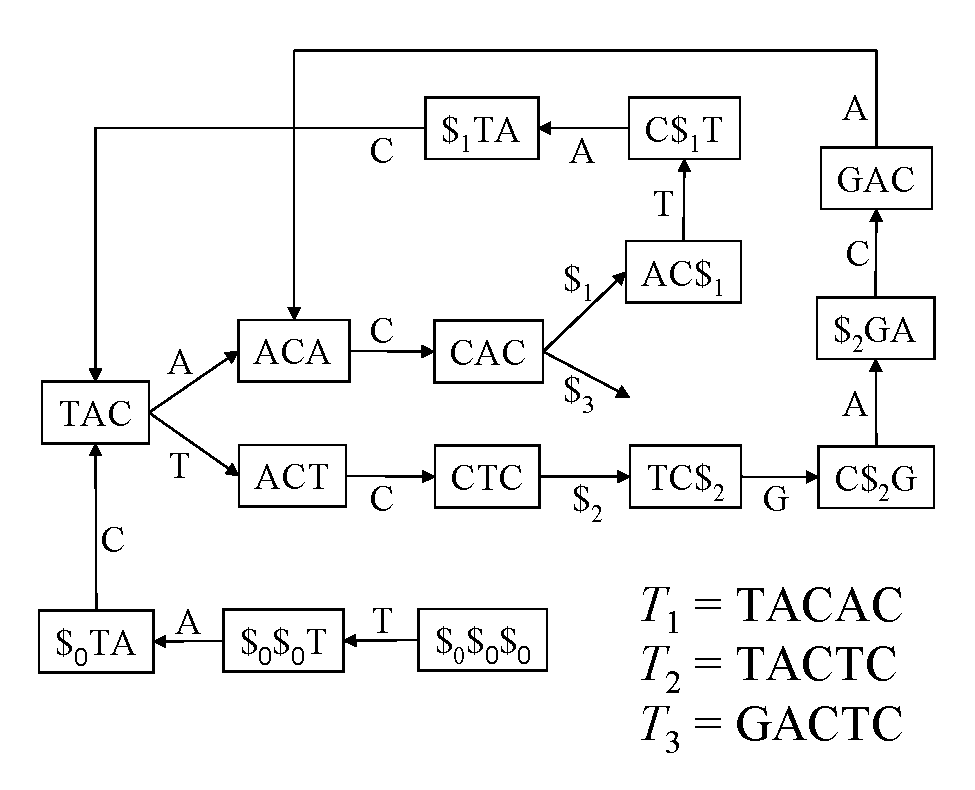
\includegraphics[scale=0.70]{fig3.eps} %PS
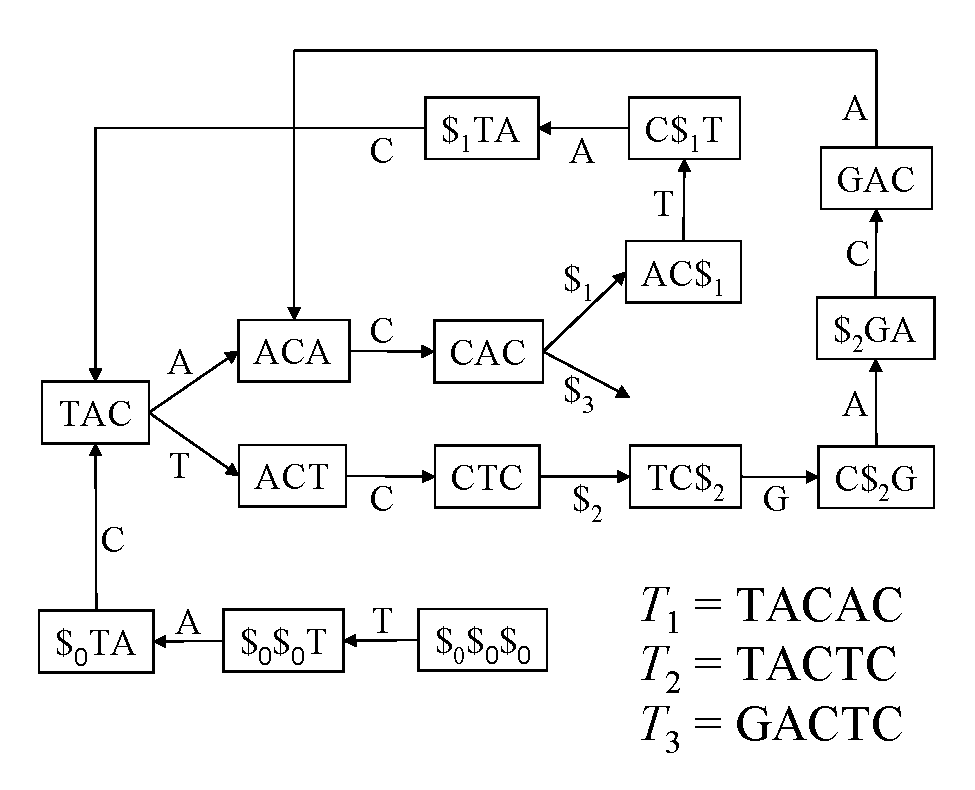
\includegraphics[scale=0.70]{fig3}
\caption{The $3$-dimensional de Bruijn graph of strings `TACAC', `TACTC', and
`GACTC'.}
\label{fig:debruijn}
\end{center}
\end{figure}

\cite{ICTFM12} introduced the {\em colored de Bruijn graph}, a variant of the classical structure, which is aimed at ``detecting and genotyping simple and complex genetic variants in an individual or population.'' The edge structure of the colored de Bruijn graph is the same as the classic structure, but now to each vertex ($(k - 1)$-mer) and edge ($k$-mer)
% FIXME: node coloring (CORTEX) looses information preserved in edge coloring(VARI), should we discuss this?  i.e. two nodes with the same color may or may not have a connecting edge with that color, but if you only color the nodes, you can't tell which is the case
is associated a list of colors corresponding to the samples in which the vertex or edge label exists. More specifically, given a set of $n$ samples, there exists a set $\mathcal{C}$ of $n$ colors $c_1, c_2, .., c_n$ where $c_i$ corresponds to sample $i$ and all $k$-mers and $(k-1)$-mers that are contained in sample $i$ are colored with $c_i$. A {\em bubble} in this graph corresponds to an undirected cycle, and is shown to be indicative of biological variation by \cite{ICTFM12}. 
{\sc Cortex}, the implementation of \cite{ICTFM12}, uses the colored de Bruijn graph to develop a method of assembling multiple genomes simultaneously, without losing track of the individuals from which $(k - 1)$-mers (and $k$-mers) originated. This graph is derived from either multiple reference genomes, multiple samples, or a combination of both.

Variant information of an individual or population can be deduced from structure present in the colored de Bruijn graph and the colors of each $k$-mer.
As implied by \cite{ICTFM12}, the ultimate intended use of colored de Bruijn graphs is to apply it to massive, population-level sequence data that is now abundant due to next generation sequencing technology (NGS) and multiplexing. These technologies have enabled production of sequence data for large populations, which has led to ambitious sequencing initiatives that aim to study genetic variation for agriculturally and bio-medically important species.  These initiatives include the {\em Genome 10K} project that aims to sequence the genomes of 10,000 vertebrate species~\citep{Haussler:2009}, the {\em iK5} project~\citep{Robinson:2011}, the 150 Tomato Genome ReSequencing project~\citep{tomato1,tomato2}, and the 1001 Arabidopsis project, a worldwide initiative to sequence cultivars of {\em Arabidopsis}~\citep{arabidopsis}.   Given the large number of individuals and sequence data involved in these projects, it is imperative that the colored de Bruijn graph can be stored and traversed in a space- and time-efficient manner.
 

\section{Rank and Select}
 \label{sec:rank} Two basic operations used in almost
every succinct and compressed data structure are {\em rank} and {\em select}.
Given a sequence (string) $S[1,n]$ over an alphabet $\Sigma =
\{1,\ldots,\sigma\}$, a character $c \in \Sigma $, and integers $i$,$j$,
$\rank_c(S,i)$ is the number of times that $c$ appears in $S[1,i]$, and
$\select_c(S,j)$ is the position of the $j$-th occurrence of $c$ in $S$.
%There is a great variety of techniques to answer these queries, with
%suitability depending on the nature of the sequence, for example, on whether or
%not it will be compressed and on the size of the alphabet.
For a binary string $B[1,n]$, the classic solution for rank and
select~\cite{Mun96} is built upon the input sequence, requiring $o(n)$
additional bits.  Generally, $\rank_1$ and $\select_1$ are considered the
default rank and select queries.  More advanced solutions
(e.g.~\cite{bitvector}) achieve zero-order compression of $B$,
%For example, the several structures (e.g.~\cite{bitvector}), (see
%also~\cite{kkp2014}), 
representing it in just $nH_0(B) + o(n)$ bits of space, and supporting $\rank$
and $\select$ operations in constant time. 
%Several practical implementations and improvements of RRR exists (see,
%e.g.,~\cite{kkp2014}).

\section{Wavelet Trees} \label{sec:WVT} To support rank and select on larger
alphabet strings, the wavelet tree~\cite{ggv2003,n2013} is a commonly used data
structure that occupies $n\log\sigma + o(n\log\sigma)$ bits of space and
supports $\rank$ and $\select$ queries in $\Oh{\log\sigma}$ time.  Wavelet trees
also support a variety of more complex queries on the underlying string (see,
e.g.~\cite{gnp2012}), in $\Oh{\log\sigma}$ time, and we will make use of some of
this functionality in Section~\ref{sec:implementing}.


%Our data structure for colored de Bruijn graphs is based on a succinct representation of individual de Bruijn graphs that was introduced by \cite{BOSS12} and which we refer to as the BOSS representation from the authors' initials.  The BOSS representation was in turn based on an adaptation of \cite{FM05} FM-indexes.  Before getting to our description of the succinct colored de Bruijn graph data structure, 
%In the rest of this section 
%we first describe FM-indexes and then explain the BOSS representation.
%Our explanation of BOSS is particularly simple and may be of independent interest to those wanting to better understand that data structure.
% This new take on BOSS was key to our development of our succinct colored de Bruijn graph. 
% Travis: No it wasn't, it came afterward. :o)

\section{FM-indexes}
\label{subsec:fm-indexes}

Consider a string $S$.  Let $F$ be the list of $S$'s characters sorted lexicographically by the suffixes starting at those characters, and let $L$ be the list of $S$'s characters sorted lexicographically by the suffixes starting immediately after those characters.  (The names $F$ and $L$ are standard for these lists.)  If \(S [i]\) is in position $p$ in $F$ then \(S [i - 1]\) is in position $p$ in $L$.  Moreover, if \(S [i] = S [j]\) then \(S [i]\) and \(S [j]\) have the same relative order in both lists; otherwise, their relative order in $F$ is the same as their lexicographic order.  This means that if \(S [i]\) is in position $p$ in $L$ then, assuming arrays are indexed from 0 and $\prec$ denotes lexicographic precedence, in $F$ it is in position
%\begin{multline*}
  \[|\{h\,:\,S [h] \prec S[i]\}| + |\{h\,:\,L [h] = S [i],\ h \leq p\}| - 1\,.\]
%  \end{multline*}
Finally, notice that the last character in $S$ always appears first in $L$.  It follows that we can recover $S$ from $L$, which is the famous Burrows-Wheeler Transform (BWT)~\citep{BW94} of $S$.

The BWT was introduced as an aid to data compression: it moves characters followed by similar contexts together and thus makes many strings encountered in practice locally homogeneous and easily compressible.  \cite{FM05} realized it could also be used for indexing because, if we know the range \(\BWT (S) [i..j]\) occupied by characters immediately preceding occurrences of a pattern $P$ in $S$, then we can compute the range \(\BWT (S) [i'..j']\) occupied by characters immediately preceding occurrences of \(c P\) in $S$, for any character $c$, since
\begin{eqnarray*}
i' & = & |\{h\,:\,S [h] \prec c\}| + |\{h\,:\,S [h] = c, h < i\}|\\
j' & = & |\{h\,:\,S [h] \prec c\}| + |\{h\,:\,S [h] = c, h \leq j\}| - 1\,.
\end{eqnarray*}
Notice \(j' - i' + 1\) is the number of occurrences of \(c P\) in $S$.  The essential components of an FM-index for $S$ are, first, an array storing \(|\{h\,:\,S [h] \prec c\}|\) for each character $c$ and, second, a rank data structure for \(\BWT (S)\) that quickly tells us how often any given character occurs up to any given position\footnote{Given a sequence (string) $S[1,n]$ over an alphabet $\Sigma = \{1,\ldots,\sigma\}$, a character $c \in \Sigma $, and an integer
$i$, $\rank_c(S,i)$ is the number of times that $c$ appears in $S[1,i]$.}.  
To be able to locate the occurrences of patterns in $S$ (in addition to just counting them), we can use a sampled suffix array of $S$ and a bitvector indicating the positions in \(\BWT (S)\) of the characters preceding the sampled suffixes.


\section{BOSS representation}
\label{sec:BOSS}

% TODO: take the concise description of BOSS from CDBG paper?

Conceptually, to build the BOSS representation~\cite{BOSS12} of a $K$th-order de Bruijn graph from a set of \((K + 1)\)-mers, we first add enough dummy \((K + 1)\)-mers starting with \$s so that if \(\alpha a\) is in the set, then some \((K + 1)\)-mer ends with $\alpha$ ($\alpha$ a $K$-mer, $a$ a symbol).  We also add enough dummy \((K + 1)\)-mers ending with \$ that if \(b \alpha\) is in the set, with $\alpha$ containing no \$ symbols, then some \((K + 1)\)-mer starts with $\alpha$.  We then sort the set of \((K + 1)\)-mers into the right-to-left lexicographic order of their first $K$ symbols (with ties broken by the last symbol) to obtain a matrix.  If the $i$th through $j$th \((K + 1)\)-mers start with $\alpha$, then we say node \([i, j]\) in the graph has label $\alpha$, with \(j - i + 1\) outgoing edges labelled with the last symbols of the $i$th through $j$th \((K + 1)\)-mers.  If there are $n$ nodes in the graph, then there are at most \(\sigma n\) rows in the matrix, i.e., \((K + 1)\)-mers.

For example, if \(K = 3\) and the matrix is the one from Bowe et al.'s paper,
shown in the left of Fig.~\ref{fig:matrix}, then the \(n = 11\) nodes are
\begin{gather*}
 [1, 1], [2, 2], [3, 3], [4, 5], [6, 6], [7, 7], [8, 9], [10,
 10], [11, 11], \\ [12, 12], [13, 13]
\end{gather*}
with labels

\begin{gather*}
 \mathrm{\$\$\$}, \mathrm{CGA}, \mathrm{\$TA}, \mathrm{GAC}, \mathrm{TAC},
\mathrm{GTC}, \mathrm{ACG}, \mathrm{TCG}, \mathrm{\$\$T}, \\
\mathrm{ACT}, \mathrm{CGT},
\end{gather*}%
respectively. The 3rd-order de Bruijn graph itself is shown in the right of the figure.

\begin{figure*}[!t]
\centering
\begin{tabular}{c@{\hspace{10ex}}c}
\begin{tabular}{r@{\hspace{1ex}}@{\hspace{1ex}}@{\hspace{1ex}}l@{\hspace{1ex}}c}
1) & \,\$\,\$\,\$\, & T\\
2) & CGA & C\\
3) & \,\$\,TA & C\\
4) & GAC & G\\
5) & GAC & T\\
6) & TAC & G\\
7) & GTC & G\\
8) & ACG & A\\
9) & ACG & T\\
10) & TCG & A\\
11) & \,\$\,\$\,T & A\\
12) & ACT & \$\\
13) & CGT & C
\end{tabular} &
\raisebox{-10ex}
{\includegraphics*[trim = 0cm 0cm 9cm 24cm, width=50ex]{images/dbg-with-dummies.pdf}}
\end{tabular}
\caption{The BOSS matrix (left) and de Bruijn graph (right) for the quadruples CGAC, GACG, GACT, TACG, GTCG, ACGA, ACGT, TCGA, CGTC.}
\label{fig:matrix}
\hrulefill
\end{figure*}

Bowe et al.\ described a number of queries on the graph, all of which can be implemented in terms of the following three with at most an $\Oh{\sigma}$-factor slowdown:
\begin{itemize}
\item $\forward(v, a)$ returns the node $w$ reached from $v$ by an edge labelled $a$, or NULL if there is no such node;
\item $\backward(v)$ lists the nodes $u$ with an edge from $u$ to $v$;
\item $\lastchar(v)$ returns the last character of $v$'s label.
\end{itemize}
In our example, \(\forward \allowbreak ([8, 9], \mathrm{A}) \allowbreak =
\allowbreak [2, 2]\),
\(\backward \allowbreak ([2, 2]) \allowbreak = \allowbreak [8, 9], [10, 10]\) and
\(\lastchar \allowbreak ([8, 9]) \allowbreak = \allowbreak \mathrm{G}\).
Since $\backward$ always returns at least one node, we can recover any non-dummy node's entire label by $K$ calls to $\lastchar$ interleaved with \(K - 1\) calls to $\backward$.




\section{Varying order}
\label{sec:changing}

If we delete the first column of the matrix in Figure~\ref{fig:matrix}, the result is {\em almost} the BOSS matrix for a 2nd-order de Bruijn graph whose nodes
\[[1, 1], [2, 2], [3, 3], [4, 6], [7, 7], [8, 10], [11, 11], [12, 12], [13, 13]\]
have labels
\[\mathrm{\$\$, GA, TA, AC, TC, CG, \$T, CT, GT}\,,\]
respectively.  Similarly, if we delete the first two columns of the original matrix, the result is almost the BOSS matrix for a 1st-order graph whose nodes
\[[1, 1], [2, 3], [4, 7], [8, 10], [11, 13]\]
have labels
\[\mathrm{\$, A, C, G, T}\,,\]
respectively.  If we delete the first three columns, the result is almost the BOSS graph for the 0th-order graph whose single node \([1, 13]\) has an empty label.  Notice we allow the same node to appear in different graphs, with labels of different lengths.  If readers find this confusing, they can imagine that nodes are triples instead of pairs, with the additional component storing the label's length.

The truncated form of a higher order BOSS differs from the BOSS of a lower order in that
%The problem is that 
some rows are repeated, which could prevent the BOSS representation from working properly.  Suppose that, instead of trying to apply $\forward$, $\backward$ and $\lastchar$ directly to nodes in the new graphs, we augment the BOSS representation of the original graph to support the following three queries:
\begin{itemize}
\item $\shorter(v, k)$ returns the node whose label is the last $k$ characters of $v$'s label;
\item $\longer(v, k)$ lists nodes whose labels have length \(k \leq K\) and end with $v$'s label;
\item $\maxlen(v, a)$ returns some node in the original graph whose label ends with $v$'s label, and that has an outgoing edge labelled $a$, or NULL otherwise. %if there is no such node.
\end{itemize}
If we want a node in the original graph whose label ends with $v$'s label but we do not care about its outgoing edges, then we write \(\maxlen(v, *)\).  Notice $\shorter$ and $\longer$ are symmetric, in the sense that if $v$'s label has length $k_v$ and \(x \in \longer(v, k_v)\), then \(\shorter(x, k_v) = v\).  In our example, \(\shorter([4, 5], 2) = [4, 6]\) while \(\longer([4, 6], 3) = [4, 5], [6, 6]\) and \(\maxlen ([4, 6], \mathrm{G})\) could return either \([4, 5]\) or \([6, 6]\), while \(\maxlen([4, 6], \mathrm{T}) = [4, 5]\) and \(\maxlen([4, 6], \mathrm{A}) = \mathrm{NULL}\).

If $v$ is a node in the original graph --- e.g., $v$ is returned by $\maxlen$ --- then we can use the BOSS implementations of $\forward$, $\backward$ and $\lastchar$.  Otherwise, if $v$'s label has length $k_v$ then
\begin{eqnarray*}
\forward(v, a) & = & \shorter(\forward(\maxlen(v, a), a), k_v)\\
\lastchar(v) & = & \lastchar(\maxlen(v, *))\,.
\end{eqnarray*}
Assuming queries can be applied to lists of nodes, we can compute \(\backward(v)\) as %by computing
\[\shorter(\backward(\maxlen(\longer(v, k_v + 1), *)), k_v),\]
removing any duplicates.

To see why we can compute $\backward$ like this, suppose $v$'s label is \(\alpha a\), so \(\longer(v, \allowbreak k_v + 1)\) returns a list of all \(d \leq \sigma\) nodes whose labels have the form \(b \alpha a\).  Applying $\maxlen$ to this list returns a second list of $d$ nodes, with labels \(\beta_1 b_1 \alpha a, \ldots, \beta_d b_d \alpha a\) of length $K$.  Applying $\backward$ to this second list returns yet a third list, of all the at most \(\sigma d\) nodes whose labels have the form \(c \beta_i b_i \alpha\).  We need only one node returned calling $\backward$ on each node in the second list, so we can discard all but at most $d$ nodes in the third list.  Finally, applying $\shorter$ to the third list returns a fourth list, of all $d$ nodes whose labels have the form \(b_i \alpha\), each of which may be repeated at most $\sigma$ times in the list.



\section{Implementing $\shorter$, $\longer$ and $\maxlen$}
\label{sec:implementing}

The BOSS representation includes a wavelet tree over the last column $W$ of the BOSS matrix, and a bitvector $L$ of the same length with 1s marking where nodes' intervals end.  In our example, \(W = \mathrm{TCCGTGGATAA\$C}\) and \(L = 1110111011111\).

%With these data structures, 
Now we can implement \(\maxlen([i, j], a)\) in $\Oh{\log \sigma}$ time: we use $\rank$ and $\select$ on $W$ to find an occurrence \(W [r]\) of $a$ in \(W [i..j]\), if there is one; we then use $\rank$ and $\select$ on $L$ to find the last bit \(L [i' - 1] = 1\) with \(i' \leq r\) and the first bit \(L [j'] = 1\) with \(j' \geq r\), and return \([i', j']\).  (If there is no occurrence of 1 strictly before \(L [r]\), then we set \(i' = 1\).)  We can implement \(\maxlen([i, j], *)\) in $\Oh{1}$ time: instead of using $\rank$ and $\select$ on $W$ to find $r$, we simply choose any $r$ between $i$ and $j$.

In our example, for \(\maxlen([4, 6], \mathrm{G})\) we first find an occurence \(W [r]\) of G in \(W [4..6]\), which could be either \(W [4]\) or \(W [6]\); if we choose \(r = 4\) then the last bit \(L [i' - 1] = 1\) with \(i' \leq r\) is \(L [3]\) and the first bit \(L [j'] = 1\) with \(j' \geq r\) is \(L [5]\), so we return \([i', j'] = [4, 5]\); if we choose \(r = 6\) then the last bit \(L [i' - 1] = 1\) with \(i' \leq r\) is \(L [5]\) and the first bit \(L [j'] = 1\) with \(j' \geq r\) is \(L [6]\), so we return \([i', j'] = [6, 6]\).

To implement $\shorter$ and $\longer$, we store a wavelet tree over the sequence $L^*$ in which \(L^* [i]\) is the length of the longest common suffix of the label of the node in the original graph whose interval includes $i$, and the label of the node whose interval includes \(i + 1\); this takes $\Oh{\log K}$ bits per \((K + 1)\)-mer in the matrix.  To save space, we can omit $K$s in $L^*$, since they correspond to 0s in $L$ and indicate that $i$ and \(i + 1\) are in the interval of the same node in the original graph; the wavelet tree then takes $\Oh{\log K}$ bits per node in the original graph and $\Oh{n \log K}$ bits in total.  In our example, \(L^* = 0, 1, 0, 3, 2, 1, 0, 3, 2, 0, 1, 1\) (and we can omit the 3s to save space).

For \(\shorter([i, j], k)\), we use the wavelet tree over $L^*$ to find the largest \(i' \leq i\) and the smallest \(j' \geq j\) with \(L^* [i' - 1], L^* [j'] < k\) and return \([i', j']\), which takes $\Oh{\log K}$ time.  For \(\longer([i, j], k)\), we use the wavelet tree to find the set \(B = \{b\,:\,L^* [b] < k\,;\,i - 1 \leq b \leq j\}\) --- which includes \(i - 1\) and $j$ --- and then, for each consecutive pair \((b, b')\) in $B$, we report \([b + 1, b']\); this takes a total of $\Oh{|B| \log K}$ time.  With these implementations, if the time bounds for \(\forward(v, a)\), \(\backward(v)\) and \(\lastchar(v)\) are $\Oh{t_\forward}$, $\Oh{t_\backward}$ and $\Oh{t_\lastchar}$ when $v$ is a node in the original graph, respectively, then they are $\Oh{t_\forward + \log \sigma + \log K}$, $\Oh{\sigma (t_\backward + \log K)}$ and $\Oh{t_\lastchar + 1}$ when $v$ is not a node in the original graph.

In our example, for \(\shorter([4, 5], 2)\) we find the largest \(i' \leq 4\) and the smallest \(j' \geq 5\) with \(L^* [i' - 1], L^* [j'] < 2\) --- which are 4 and 6, respectively --- and return \([4, 6]\).  For \(\longer([4, 6], 3)\) we find the set \(B = \{b\,:\,L^* [b] < 3\,;\,3 \leq b \leq 6\} = \{3, 5, 6\}\) and report \([4, 5]\) and \([6, 6]\).

A smaller but slower approach is not to store $L^*$ explicitly but to support access to any cell \(L^* [i]\) by finding the nodes in the original graph whose intervals include $i$ and \(i + 1\), then using $\backward$ and $\lastchar$ to compute their labels and find the length of their longest common suffix; this takes a total of $\Oh{K (t_\backward + t_\lastchar)}$ time.  To implement $\shorter$ and $\longer$, we store a range-minimum data structure~\cite{fh2011} over $L^*$, which takes \(2 n + o (n)\) bits and returns the position of the minimum value in a specified substring of $L^*$ in $\Oh{1}$ time.

For \(\shorter([i, j], k)\), we use binary search and range-minimum queries to find the largest \(i' \leq i\) and the smallest
\(j' \geq j\) with \(L^* [i' - 1], L^* [j'] < k\) and return \([i', j']\), which takes $\Oh{K (t_\backward + t_\lastchar) \log (n \sigma)}$ time. 
%(With a more complicated use of the range-minimum data structure, which we will describe in the full version of this paper, we use $\Oh{K^2 (t_\backward + t_\lastchar)}$ time.)
For \(\longer([i, j], k)\), we recursively split \([i, j]\) into subintervals with range-minimum queries, at each step using $\backward$ and $\lastchar$ to check that the minimum value found is less than $k$; this takes $\Oh{K (t_\backward + t_\lastchar)}$ time per node returned.  With these implementations, \(\forward(v, a)\), \(\backward(v)\) and \(\lastchar(v)\) take $\Oh{t_\forward + K (t_\backward + t_\lastchar) \log (n \sigma)}$, $\Oh{\sigma K (t_\backward + t_\lastchar) \log (n \sigma) + \sigma^2 t_\backward}$ and $\Oh{t_\lastchar + 1}$ time, respectively, when $v$ is not a node in the original graph.

For \(\sigma = \Oh{1}\), our bounds are summarized in the following theorem. % We will provide more details in the full version of this paper.

\begin{theorem}
\label{thm:bounds}
When \(\sigma = \Oh{1}\), we can store a variable-order de Bruijn graph in $\Oh{n \log K}$ bits on top of the BOSS representation, where $n$
is the number of nodes in the $K$th-order de Bruijn graph, and support \forward\ and \backward\ in $\Oh{\log K}$ time and \lastchar\ in
$\Oh{1}$ time.  We can also use $\Oh{n}$ bits on top of the BOSS representation, at the cost of using $\Oh{K \log n / \log \log n}$ time
for \forward\ and \backward.
\end{theorem}

%shorter - logK
%longer - |B| log K time (for a set of B resulting nodes)

%K^2 log^2 n / log log n

%O(B K^2 log^2 n / log log n)

\chapter{Experimental Analysis}
\label{sec:experiments}

\section{Implementation}
SDSL-lite, STXXL for the implementation of on disk sorting, which also lets the user specify the work to be done in memory.

%\section{Primary vs Secondary memory construction}
%In memory, single IDE disk, single SSD, 2 SSDs, 4 SSDs.
%Cost effective? SSD vs memory cost.

\section{BOSS vs Competing methods}
Construction time, bits per edge, and traversal time for 2 small genomes.
(would have to implement simple traversal for this)

\section{Variable-order vs fixed-order}
\input{chapters/experiments-varord.tex}


%%%%%%%%%%%%%%  PS
\section{Cortex vs Vari}
%Measure full runtime of both.
%Test w/ on disk colour matrix? (sort indices after traversal)
\pyt{Remove the initial 2 sentences? I.e. Measure full runtime of both...}


We evaluated $\ours$ on five different datasets, described below.  For performance evaluation, we compare peak memory, which was measured as the maximum resident set size, and runtime, measured as the user process time as our metrics.  In addition to evaluating performance, we also validated $\ours$ by the ability to correctly call bubbles and to accurately identify the origin of $k$-mers in a simulated metagenomics sample.  Finally, we present observations computed by $\ours$ on a collection of metagenomic samples taken from commercial beef production facilities.



\subsection{Datasets} \label{data}

Five different datasets were chosen in order to test and evaluate $\ours$ on a variety of diverse yet realistic data types that are likely to be used as input into $\ours$.  The first dataset contained six sub-strains of the {\em E. coli} K-12 strain reference genomes from NCBI.  The accession and substrains are 	AP009048 -- W3110,  
	CP009789 -- ER3413, 
	CP010441 -- ER3445, 
	CP010442 -- ER3466, 
	CP010445 -- ER3435, and 
	U00096   -- MG1655. 
    Each of the genomes contained approximately 4.6 million base pairs and had a median GC content of 49.9\%.

% (\ref{tbl-ecoli}).


    
%% \begin{table}[h!]
%%   \small
%%   \centering
%%   \begin{tabular}{c|c|c}
%% 		{\bf Accession Number}		& {\bf Sub-strain}	& {\bf Genome Size} 	 \\
%% 	\hline
%% 	\hline
%% 	AP009048 & W3110  & 4,646,332 bp \\
%% 	CP009789 & ER3413 & 4,558,660 bp \\
%% 	CP010441 & ER3445 & 4,607,634 bp \\
%% 	CP010442 & ER3466 & 4,660,432 bp \\
%% 	CP010445 & ER3435 & 4,682,086 bp \\ 
%% 	U00096   & MG1655 & 4,641,652 bp\\
%%  	\end{tabular}
%%       \caption{Characteristics of the substrains of \emph{E. coli} K-12 used to test the performance and accuracy of $\ours$}.
%%  \label{tbl-ecoli}
%% \end{table}

Our second dataset was composed of reference genomes for four different plant species: \emph{Oryza sativa Japonica} (rice, NCBI Accession numbers: NC\_008394 to NC\_008405), \emph{Solanum lycopersicum} (tomato, NCBI Accession numbers: NC\_015438 to NC\_015449),  \emph{Zea mays} (corn, NCBI Accession numbers: NC\_024459 to NC\_024468), and  \emph{Arabidopsis thaliana} (Arabidopsis, [NCBI Accession numbers: NC\_003070 to NC\_003076).  The genome sizes and GC content were 430 Mbp and 43.42\% \citep{rice}, 950 Mbp and 43.42\% \citep{tomato1,tomato2}, 2.07 Gbp and 35.70\% \citep{corn}, and 135 Mbp and 47.4\% \citep{swarbreck}, respectively.  Hence, this represents a significantly larger dataset with more varied GC content than the {\em E. coli} dataset, and therefore placed more demands on both the performance and accuracy of $\ours$.  


%% \begin{table}[h!]
%%   \small
%%   \centering
%%   \begin{tabular}{c|c|c}
%% 		{\bf AMR Gene}&{\bf Resistance Type}&{\bf Accession Number} 	 \\
%% 	\hline
%% 	\hline
%% 	AmpH & beta-lactamase & AFQ67211 \\
%% 	OKP-B-4 & beta-lactamase & CAJ19612 \\
%% 	NDM-6 & beta-lactamase  & AEX08599 \\
%% 	MAL-1 & beta-lactamase & CAC33434  \\
%% 	MOX-2 & beta-lactamase  & CAB82578  \\
%% 	TLA-1 & beta-lactamase & ADM26831   \\
%% 	SED-1 & beta-lactamase  & AAK63223   \\
%% 	TEM-1& beta-lactamase  & AFI61435   \\
%% 	TET-X & Tetracycline & AAA27471   \\
%% 	TET-X(1) & Tetracycline  & ADD83116 \\
%% 	TET-C & Tetracycline  & NP\_387454  \\
%% 	TETR-G & Tetracycline & AAB24797 \\
%%  	\end{tabular}
%%       \caption{List of AMR genes used to generate the simulated sample. The first seven genes were included in the the 54 beta-lactamase genes we considered for this experiment, and the remaining four were tetracycline genes. Each of the genes were approximately 1,000 bp in length and had varied GC content.}
%%  \label{tbl-amr}
%% \end{table}








Our third dataset consists of the set of all 3,765  NCBI GenBank assemblies having the organism\_name field equal to ``Escherichia coli'' as of March 22, 2016.  The union of all assemblies contains 155,449,228 31-mers.  The minimum, maximum, and average assembly lengths are 2,911,360 bp, 7,687,202 bp, and 5,156,744 bp, respectively.  The average GC content is 50.5\%. 

As previously described, our fourth dataset contains 54 beta-lactamase genes from a custom database and a simulated metagenomics sample.  We first compiled a database of known AMR genes based on sequences in the databases CARD \citep{mcarthur}, Resfinder \citep{zankari} and ARG-ANNOT \citep{gupta}---each of these AMR-specific databases are actively curated and contain the genetic sequences for a large variety of AMR genes.  This database contains all known AMR genes, their drug resistance, and mechanism conferring resistance.  We selected 54 beta-lactamase genes from this database that are known to have very high clinical and public health importance, and simulated 26,516,559 paired-end 120 bp reads from seven of the 54 beta-lactamase genes (Accession numbers AFQ67211, CAJ19612, AEX08599, CAC33434, CAB82578, ADM26831, AAK63223, and AFI61435), as well as four additional AMR genes that were not included in this set of 54 genes (Accession numbers AAA27471, ADD83116, NP\_387454, and AAB24797).  These latter four genes were tetracycline-resistant genes.  Tetracyclines are a group of broad-spectrum antibiotics and hence, their resistance is also clinically important.   This AMR dataset was used not only in the memory and time performance but also used to test the ability of $\ours$ in identifying beta-lactamase genes from a typical metagenomic sample containing a variety of AMR genes.  %Table \ref{tbl-amr} contains the gene name, resistance type (beta-lactamase or  tetracycline), and accession number of 11 genes that were used in simulation of the sample. 


Our fifth dataset consists of 87 metagenomic samples taken from various locations along the production process for eight pens of cattle in two beef production facilities by \cite{noyes2016resistome}.  These locations were feedlot arrival, feedlot exit, transport truck, slaughter holding (arrival), and slaughter trimmings and sponges (exit).  Samples were arranged into groups based on these locations. These samples were collected to explore the hypothesis that widespread use of antimicrobial drugs (administered with livestock feed for these samples) introduce selective pressure on microbial communities and thus foster the evolution of antimicrobial resistant bacteria.  These antimicrobial resistant bacterial are important because they present a public health risk.  In addition to the metagenomic samples, we included 4,062 AMR genes from the previously mentioned gene databases.  23 genes in the databases containing IUPAC codes other than the four bases were filtered out as KMC2 and the succinct de Bruijn graph were configured with a four symbol alphabet.  The union of all samples and genes contains 40,995,794,366 32-mers and the GC content is 44.3\%.





% software configuration
We ran our experiments with the following configuration and environment.  On the {\it E. coli} reference, plant, and simulated metagenomic datasets we ran $\ours$ with RRR encoding, without external construction, and used {\sc Cortex} as the front end to generate the uncompressed $k$-mer union and colors.  On the {\it E. coli} assembly dataset, we ran $\ours$ similarly but used the KMC2 front end and our streaming based set-union construction.  On the metagenomic sample, we ran $\ours$ with the KMC2 front end, online Elias-Fano encoding for $C$, and external BOSS construction.
% hardware configuration
The first, second, and fourth experiments were performed on a 2 Intel Xeon  E5-2650 v2 server with 386 GB of RAM, and both resident set size and user process time were reported by the operating system.  The third experiment was performed on an AMD Opteron  6220  with 512 GB of RAM and 32 cores.  The fifth experiment was performed on an AMD Opteron 6378  with 512 GB of RAM and 64 cores. 

\subsection{Time and Memory Usage}

% what is bubble calling
To compare $\ours$ resource use with {\sc Cortex} by \cite{ICTFM12}, we constructed the colored de Bruijn graph for the {\it E. coli} reference dataset, the four plant assembly dataset, and the simulated AMR dataset, then performed {\em bubble calling} on all three data structures,  and recorded the peak memory usage and runtime.    Resource comparison with {\sc Cortex} was only possible on the smaller three datasets, as the largest two have too many $k$-mers and colors to fit in memory on our machines with {\sc Cortex}.  Based on the data structure defined in {\sc Cortex}'s source as well as the supplementry information provided by Iqbal {\it et al.}, it would have required $>$ 3 TB of RAM and $>$ 18 TB of RAM for its hash table entries alone, respectively.




% construction statistics
%For the {\it E. coli} assembly dataset, after $k$-mer counting with KMC2, construction took 16 hours and 387 GB of RAM for this dataset. For the beef safety samples, it took KMC2 34 hours and 12 GB of RAM to $k$-mer count the 887 GB of trimmed reads. $\ours$ required 87 hours, 218 GB of RAM, and 4.4 TB of external memory to build the succinct colored de Bruijn graph.  The uncompressed $C$ temporary file was 1.4 TB in size, which compressed to 196 GB with Elias-Fano encoding.



%For the simulated metagenomic dataset, each AMR gene was assigned a separate color allowing the match-color algorithm to be applied.  Thus no graph traversal times are reported although the size of the structures are reported.  
%We ran the bubble calling algorithm between the colors for the assemblies ``GCF\_000005845.2\_ASM584v2\_genomic'' and ``GCF\_000006665.1\_ASM666v1\_genomic''.

%% On the final two datasets, the simulated metagenomic sample and beef safety samples, we are interested in detecting the presence of known AMR genes among the reads.  
%% we explore the feasibility of using a colored de Bruijn graph for AMR gene detection among metagenomic samples.
%% We do so by visiting $k$-mers found in AMR genes and look for those that co-occur in the metagenomic samples.

%% % discussion of k-mer intersection
%% On the final two datasets, instead of using either of {\sc Cortex}'s bubble calling algorithms, which are designed for variant detection we are interested in presence of the AMR genes in the sample.  Variants may represent read errors or largely homologous genes missing the antibiotic resistant determinant. in samples taken from a pair of individuals or individual and reference,   In this applications, instead of looking for variants, we are looking for similarity
%% % varants -- regions that differ flanked by homologous regions, we are looking strictly for homologous regions -- as the metagenomic sample may be plagued with incomplete coverage
%% in the presence of incomplete coverage, a mix of many individuals, thus weakening common read error correction assumptions, and significant homology among AMR genes and their possibly co-occuring ancestral variants leading to more tangled graphs which impair {\sc Cortex}'s cleaned individual oriented algorithm.  In the absence of a colored, metagenomic-aware traversal algorithm, we focus only on regions of similarity and allow unlimited sized gaps between them, where the metagenomic sample color may be highly tangled or unconnected.  

%% One thing that distinguishes such datasets from pangenomic datasets, such as those targeted by the bloom filter trie, is that these datasets may have significantly smaller amounts of redundancy.  On the beef safety dataset, for example, two thirds of $k$-mers occur with multiplicity of one across the whole collection.  

%% On the simulated metagenomic dataset, 

%% For the $k$-mer set operation was not necessary and no time comparison is reported.

%% Hence this experiment demonstrates the viability of AMR gene detection via $k$-mer set operations.

%% For the 87 metagenomic sample dataset, the full data structures were loaded in memory, however only the length of each gene sequence need be traversed, resulting in the relatively fast 21 minute load and traverse time compared with bubble calling across a genome.


%% On the 87 beef safety sample, we implemented a variant of {\sc Cortex}'s path divergence algorithm, which locates bubbles where one arm of the bubble is allowed to have branches because its path is guided by a reference sequence.  In our version, we traverese the walk specified by each AMR gene sequence and count the number of edges shared with all samples from each sample location in the beef production pipeline.  


%% We note the benefit  of using a rank-select capable dictionary datastructure such as RRR or Elias-Fano encoded bit vector and storing the color matrix in linearized row major order.  Samples were arranged such that all samples taken from the same location within the production process were placed in consecutive columns in $C$.
%% %To analyze colored de Bruijn graphs with {\sc Cortex}'s algorithms, we must do all pairs comparisons or at least compare every sample of interest against some reference color; both of which become a growing runtime burden as the number of colors increases.
%% In this configuration, our data structure allows us to work on groups of samples at a time while still maintaining each sample individuality for analyses when that is of interest.  Specifically, if colors are ordered by relevant groups, such as by  the location samples were taken in the beef production pipeline.  With such grouping, we can count the number of sample colors from a group that are present in a given edge quickly.  This is computed in constant time as the difference between rank queries on the group's column interval bounds.

In order to test performance characteristics, various experiments were performed on all five datasets described in the previous subsection.  Datasets varied in the number of $k$-mers in the graph from four million to over 40 billion.  As can be seen in Table \ref{tbl-cosmo}, where directly comparable, $\ours$ used less than one-fifth of the peak memory that {\sc Cortex}  required but required greater running time.  This memory and time trade-off is important in larger population level data.  %Given that {\sc Cortex} requires 100.93 GB of space for four plant species, it would be perceptibly infeasible to run it on the i5K initiative dataset that contains the genetic sequence data for 5,000 insect species.
This is highlighted by our largest two datasets which could not be run with {\sc Cortex}.
Hence, lowering the memory usage in exchange for higher running time deserves merit in contexts where there is data from large populations. 
 
%We note that the ratios were greater for the AMR dataset, which was likely due to the greater number of colors in the AMR versus the \emph{E. coli} and plant datasets (55 versus 6 and 4, respectively).


\begin{table*}%[h!]
  \small
  \centering
  \begin{tabular}{| l | r | r | c | c | c |c |}
   	\hline
	\multicolumn{1}{|l}{}
   	& \multicolumn{1}{r}{}	
	& \multicolumn{1}{r}{} 
	& \multicolumn{2}{c|}{{\sc Cortex}} 
	& \multicolumn{2}{|c|}{$\ours$}  \\
	\hline
	 Dataset & No. of $k$-mers & Colors & Memory & Time & Memory & Time \\
	\hline
	\emph{E. coli} reference genomes			& 4,627,104 		& 6 	& 363.64 MB 	& 9 s 	& 72.38 MB  	& 1m 19s\\
	Plant reference genomes					& 1,621,663,030 	& 4 	& 100.93 GB 	& 2h 18m	& 19.46 GB 	& 17h 28m\\
    NCBI \emph{E. coli} assemblies          & 155,449,228       & 3,765 & N/A        & N/A      &  26.50 GB      & 11h \\
	AMR genes and sample 					& 9,348,365 		& 55 	& 7.08 GB 	& 2m 55s	& 0.718 GB 	& 29m 21s \\ 
    Beef safety                             & 40,995,794,366    & 88    & N/A        & N/A   & 245 GB     & N/A \\
 	\hline
	\end{tabular}
  \caption{Comparison between the peak memory and time usage required to store all the $k$-mers and run bubble calling on the data in {\sc Cortex} and $\ours$.
    %$k= 31$ was used for all datasets.
    The peak memory is given in megabytes (MB) or gigabytes (GB). The running time is reported in seconds (s), minutes (m), and hours (h).}
 \label{tbl-cosmo}
\end{table*}

\subsection{Validation on E. coli Genomes}

In order to validate our data structure and test the accuracy of the bubble calling method of $\ours$, we compared the bubbles found by running the bubble calling algorithm on the \emph{E. coli} reference dataset using {\sc Cortex} and $\ours$.  The bubbles outputted by each method were compared by identifying the flank preceding each bubble.  Both $\ours$ and {\sc Cortex} identified 465 bubbles across all six \emph{E. coli} K-12 substrains.  This number accounts for the reverse complement bubbles found by $\ours$. The methods agree on 98.5\% (458 / 465) of the bubbles. Thus, $\ours$ found seven bubbles that were not identified by {\sc Cortex}, which were shown to be valid, and {\sc Cortex} found seven bubbles not identified by $\ours$.
% I'm commenting this next line out because it doesn't make sense; cortex stores connonical k-mers, so implicitly has revcomps too.
% These latter bubbles were missed by $\ours$ because the addition of the reverse complement adds complexity to the graph, which changes these regions from containing a single bubble to a more complex structure.
Nonetheless, our validation shows that 98.5\% of the variation determined by {\sc Cortex} and $\ours$ is identical.

\subsection{Validation on AMR Dataset}

Next, we validated the ability of $\ours$ to correctly identify the AMR genes contained in a metagenomics sample using a set of reference genes. $\ours$ constructed the colored de Bruijn graph from the set of 54 beta lactamases and the simulated metagenomics sample. Hence, there were 55 unique colors in the graph because there exists one color for the metagenomic sample and one unique color for each of the 54 beta-lactamase genes.  Next, for each of the 54 genes, the unique $k$-mers were identified and the total number of these $k$-mers that were contained in the simulated sample was determined.  

%Table \ref{amr2} in the Supplement gives the total number of each unique $k$-mers for each gene, the number of these $k$-mers that were found in the simulated reads, and the {\em shared k-mer fraction} that is defined by the division of the two numbers.
The shared $k$-mer fraction for each of the 54 genes ranged from 0.41 to 1 with a mean of 0.62.  All of the seven beta-lactamase genes that were contained in the simulated sample had a shared $k$-mer fraction of 1, whereas none of the remaining 47 genes did.  Of the 47 beta-lactamase genes that were not contained in the simulated sample, two had a shared $k$-mer fraction 0.98 and 0.95, however, these genes had 97\% and 95\% sequence similarity to one of the seven genes contained in the sample.  All the remaining 45 genes had a shared $k$-mer fraction between 0.79 and 0.41.  Hence, this demonstrates (on a small scale) that this use of the colored de Bruijn graph and our match color algorithm is a viable method to identify AMR genes in a metagenomics sample. 

\subsection{Observations on Beef Safety Dataset}

%While the primary purpose of this experiment is to measure the performance in terms of memory footprint, we can examine the data we collected during traversal which may be useful to biologists and spawn hypotheses for further investigation.
Finally, we used $\ours$ to make observations about the presence of AMR genes in the beef safety dataset.  As previously described, during out path divergence derived algorithm, we compute a count of how many $k$-mers in each AMR gene are found across all samples within a sample group.  This algorithm need only traverse the AMR genes, so despite the size of the overall dataset, it only took 21 minutes to load and access the necessary parts of the data structure.  In contrast, if bubble calling were to run at the same rate for this dataset as for the {\it E. coli} assembly dataset, it would take 3,001 hours to complete, thus suggesting a need for a targeted inquiry approach on datasets of this size.  

Since longer genes have more $k$-mers, the counts are likely to be larger, as are those from larger sample groups.  To make these counts comparable, we normalize by both gene length and sample group size.  We can then examine the number of genes having a disproporitionately large ($>$ 3 std. dev. above mean) shared $k$-mer count for each gene and sample group combination.  The number of such genes with disproporitionately large normalized counts in each sample group were:  feedlot arrival --- 304, feedlot exit --- 93, transport truck --- 230, slaughter holding (arrival) --- 16, and slaughter trimmings and sponges (exit) --- 0.
%Despite biases in the sampling process that need to be taken into account for substantial biological implications, one validating property of these observations is that there were no AMR genes with disproporitionately large representation in the samples taken on exit from the slaughter location.
This observation supports the conclusion of \cite{noyes2016resistome}, namely, that antimicrobial interventions during slaughter were effective in reducing AMR gene presence in the finished product. 

%\subsection{Hypotheses}
%\subsection{Method}
%\subsection{Test Data}
%\label{sec:data}

\section{Discussion and Conclusions} \label{sec:discussion} 

%To the best of our knowledge, t
This paper describes the first non-proprietary computational method for identifying misassembly errors using short read sequence data and optical mapping data.
% has not been previously considered using non-proprietary software.  
 Our results demonstrate: (1) a substantial number of misassembly errors can be identified in draft genomes of prokaryote and eukaryote speices; (2) our method scales to large genomes; and (3) it can be used in combination with any
 assembler and thus, making it a viable post-processing step for any assembly. 

While $\sequel$ is capable of identifying a significant percentage of misassembly errors, it does not address 
%the additional problem of re-assembling 
the reassembly of those the misassembled contigs. 
Correcting misassembly errors by segmenting the contigs at their breakpoints will remove the errors but will also 
%have the detrimental effect of reducing 
reduce
the N50 
of the assembly.  
For this reason, we believe that creating a reassembly tool to correctly reassemble contigs using the misassembly information and data warrants future investigation.
%Related to this problem is that of distinguishing between locally misassembled contigs and extensively misassembled contigs, which also deserves consideration.
%Hence, since SEQuel~\cite{sequel} is capable of correcting small indels and substitution errors, and $\sequel$ has the added virtue of identifying larger misassembly errors, the remaining step is to reassemble these contigs so that N50 is not degraded

While our main contributions are the computational method itself and the demonstration that optical mapping can have significant benefit for misassembly detection, optimal results are contingent upon good enzyme selection. 
Thus, we conclude by suggesting that efficient algorithmic selection of enzymes that will yield such informative optical maps in a {\em de novo} scenario is an area for interesting and important future work.  


%Moreover, the development of more sophisticated approaches to missassembly verification using optical mapping than just the presence or absence of alignments may further improve upon the results in this paper. Potential approaches include considering consistent estimated alignment loci in the genome across all optical maps, and determining the existence of unique, non-overlapping placement of each correctly assembled contig.

% We may want to add somewhere that some applications may prefer a method that favors good TPR vs FPR or vice versa and that while we've focused on a good balance, different alignment thresholds (or delta values for sequel) and combination strategies can shift this balance.






% An example of a floating figure using the graphicx package.
% Note that \label must occur AFTER (or within) \caption.
% For figures, \caption should occur after the \includegraphics.
% Note that IEEEtran v1.7 and later has special internal code that
% is designed to preserve the operation of \label within \caption
% even when the captionsoff option is in effect. However, because
% of issues like this, it may be the safest practice to put all your
% \label just after \caption rather than within \caption{}.
%
% Reminder: the "draftcls" or "draftclsnofoot", not "draft", class
% option should be used if it is desired that the figures are to be
% displayed while in draft mode.
%
%\begin{figure}[!t]
%\centering
%\includegraphics[width=2.5in]{myfigure}
% where an .eps filename suffix will be assumed under latex, 
% and a .pdf suffix will be assumed for pdflatex; or what has been declared
% via \DeclareGraphicsExtensions.
%\caption{Simulation results for the network.}
%\label{fig_sim}
%\end{figure}

% Note that the IEEE typically puts floats only at the top, even when this
% results in a large percentage of a column being occupied by floats.
% However, the Computer Society has been known to put floats at the bottom.


% An example of a double column floating figure using two subfigures.
% (The subfig.sty package must be loaded for this to work.)
% The subfigure \label commands are set within each subfloat command,
% and the \label for the overall figure must come after \caption.
% \hfil is used as a separator to get equal spacing.
% Watch out that the combined width of all the subfigures on a 
% line do not exceed the text width or a line break will occur.
%
%\begin{figure*}[!t]
%\centering
%\subfloat[Case I]{\includegraphics[width=2.5in]{box}%
%\label{fig_first_case}}
%\hfil
%\subfloat[Case II]{\includegraphics[width=2.5in]{box}%
%\label{fig_second_case}}
%\caption{Simulation results for the network.}
%\label{fig_sim}
%\end{figure*}
%
% Note that often IEEE papers with subfigures do not employ subfigure
% captions (using the optional argument to \subfloat[]), but instead will
% reference/describe all of them (a), (b), etc., within the main caption.
% Be aware that for subfig.sty to generate the (a), (b), etc., subfigure
% labels, the optional argument to \subfloat must be present. If a
% subcaption is not desired, just leave its contents blank,
% e.g., \subfloat[].


% An example of a floating table. Note that, for IEEE style tables, the
% \caption command should come BEFORE the table and, given that table
% captions serve much like titles, are usually capitalized except for words
% such as a, an, and, as, at, but, by, for, in, nor, of, on, or, the, to
% and up, which are usually not capitalized unless they are the first or
% last word of the caption. Table text will default to \footnotesize as
% the IEEE normally uses this smaller font for tables.
% The \label must come after \caption as always.
%
%\begin{table}[!t]
%% increase table row spacing, adjust to taste
%\renewcommand{\arraystretch}{1.3}
% if using array.sty, it might be a good idea to tweak the value of
% \extrarowheight as needed to properly center the text within the cells
%\caption{An Example of a Table}
%\label{table_example}
%\centering
%% Some packages, such as MDW tools, offer better commands for making tables
%% than the plain LaTeX2e tabular which is used here.
%\begin{tabular}{|c||c|}
%\hline
%One & Two\\
%\hline
%Three & Four\\
%\hline
%\end{tabular}
%\end{table}


% Note that the IEEE does not put floats in the very first column
% - or typically anywhere on the first page for that matter. Also,
% in-text middle ("here") positioning is typically not used, but it
% is allowed and encouraged for Computer Society conferences (but
% not Computer Society journals). Most IEEE journals/conferences use
% top floats exclusively. 
% Note that, LaTeX2e, unlike IEEE journals/conferences, places
% footnotes above bottom floats. This can be corrected via the
% \fnbelowfloat command of the stfloats package.

\section*{Acknowledgments}
We thank two anonymous reviewers for thoughtful comments that materially improved this manuscript.


% Can use something like this to put references on a page
% by themselves when using endfloat and the captionsoff option.
\ifCLASSOPTIONcaptionsoff
  \newpage
\fi



% trigger a \newpage just before the given reference
% number - used to balance the columns on the last page
% adjust value as needed - may need to be readjusted if
% the document is modified later
%\IEEEtriggeratref{8}
% The "triggered" command can be changed if desired:
%\IEEEtriggercmd{\enlargethispage{-5in}}

\bibliographystyle{IEEEtran}
\bibliography{IEEEabrv,dbg}

% You can push biographies down or up by placing
% a \vfill before or after them. The appropriate
% use of \vfill depends on what kind of text is
% on the last page and whether or not the columns
% are being equalized.

%\vfill

% Can be used to pull up biographies so that the bottom of the last one
% is flush with the other column.
%\enlargethispage{-5in}

\end{document}


